\chapter{Implementazione e prove sperimentali}

In questo capitolo verranno presentate le caratteristiche tecnologiche dei veicoli utilizzati nella fase sperimentale, le proprietà fisiche di ogni scenario modellato e le varie misure di qualità.

Per ogni scenario verrà illustrata la complessità ambientale, insieme alla rappresentazione reale ed al modello della relativa mappa, per comprendere le caratteristiche morfologiche dell'area e la strattura degli ostacoli presenti.
Verranno, inoltre, analizzate le informazioni relative ai parametri utilizzati nella fase di ottimizzazione e adattamento delle metaeuristiche alla missione.
 
Infine, i risultati sperimentali verranno presentati alla fine di ogni scenario ed alla fine del capitolo per un'analisi comparativa con i risultati già presenti in letteratura.

Nel caso dello scenario \textit{Illegal Dump} sono state adattate entrambe le strategie di esplorazione analizzate nei capitoli precedenti e la strategia di reclutamento di Sciadro 3.2, per dimostrare la possibilità di adattare strategie con diversi livelli di astrazione.
Nel caso degli scenari \textit{Rural Mine} e \textit{Urban Mine}, invece, l'adattamento interessa solo la strategia di esplorazione di Sciadro 3.2, al fine di comparare le performance del simulatore, ed in particolare del modulo di ottimizzazione parametrica, con quelle ottenute in \cite{cimino2019adaptive}, nel quale l'ottimizzazione parametrica è implementata in Matlab.
A tal proposito, nelle sezioni dedicate alla comparazione di questi approcci, indicheremo con \textit{Sciadro 3.2} il simulatore analizzato in questo documento e con \textit{Sciadro 3.1} l'ambiente di simulazione analizzato in \cite{cimino2019adaptive}.

\section{Specifiche tecniche del drone}

Le caratteristiche ambientali dei vari scenari sono state prese in considerazione per le specifiche tecniche degli UAV disponibili in commercio. 
La tecnologia selezionata per modellare gli agenti responasbili del completamento della missione è la seguente:
\begin{itemize}
    \item \textit{Modello drone:} Dji Matrice M200
    \item \textit{Sensore di rilevamento:} Dji Zenmuse XT2 (Visual + Thermal Camera) 
\end{itemize}
Tale tecnologia è stata adottata sulla base delle conoscenze e delle competenze acquisite in diversi progetti che utilizzano la tecnologia UAV per il monitoraggio e la sorveglianza ambientale. 
In particolare, la tecnologia di rilevamento proposta, si basa su \cite{persechino2010aerospace} e \cite{lega2012using};

\begin{figure}[H] 
    \captionsetup{justification=centering, margin=2cm, font=footnotesize}
    \begin{center}
    \makebox[\textwidth]{\includegraphics[width=0.4\paperwidth]{img/dji_matrice_sensore.jpg}}
    \end{center}
    \caption{Rappresentazione del drone Dji Matrice M200 equipaggiato con il sensore Dji Zenmuse XT2.}
    \label{dji_matrice}
\end{figure}

Le tabelle \ref{tabella_tecnologia_drone} e \ref{tabella_tecnologia_sensore}, invece, mostrano, rispettivamente, la configurazione parametrica relativa alle specifiche del drone  \cite{matrice200} e le apparecchiature di sensing utilizzate in fase di simulazione.

\begin{table}[H]
    \centering
    
    \begin{tabular}{|l|c|}
    \hline
    \textbf{Parameter}              & \textbf{Value}                \\ \hline
    Radius                          & $0.3 \; m$                    \\ \hline
    Max speed                       & $17 \; m/s$                   \\ \hline
    Max acceleration                & $4.4 \; m/s^{2}$              \\ \hline
    Max angular speed               & $2.6 \; rad/s$                \\ \hline
    Max angular acceleration        & $7 \; rad/s^{2}$              \\ \hline
    Battery duration                & $24 \; min$                   \\ \hline
    Obstacle vision distance        & $3-30 \; m$                   \\ \hline
    Obstacle vision angle           & $60 \; \circ$                     \\ \hline
    \end{tabular}%
    
    \caption{Specifiche tecniche del modello di drone \textit{Dji Matrice 200}.}
    \label{tabella_tecnologia_drone}
\end{table}

\begin{table}[H]
    \centering
    
    \begin{tabular}{|c|c|c|}
    \hline
    \begin{tabular}[c]{@{}l@{}}\textbf{Sensing} \\ \textbf{technology}\end{tabular}                   & \textbf{Sensor model}                 & \begin{tabular}[c]{@{}l@{}}\textbf{Sensing} \\ \textbf{radius}\end{tabular}        \\ \hline
    \begin{tabular}[c]{@{}l@{}}Visual + \\ Thermal\end{tabular}                              & Dji Zenmuse XT2                       & 5 m                            \\ \hline    
    \end{tabular}%    
    \caption{Specifiche tecniche dell'equipaggiamento di sensing.}
    \label{tabella_tecnologia_sensore}
\end{table}

\section{Scenario \textit{Illegal Dump}}

In questa sezione sono illustrati lo scenario utilizzato e le varie misure di qualità. 
Lo scenario è statico: \textit{Illegal Dump} si basa sulla mappa di una discarica abusiva di Paternò, Italia \cite{trashout2018}.
Di seguito sono riportate le caratteristiche dello scenario:

\begin{itemize}
    \item \textit{Area in metri:} 400 x 400
    \item \textit{Area in patch:} 201 x 201
    \item \textit{Dimensione patch:} 1.99m x 1.99m
    \item \textit{Conversione spaziale:} 1 m = 0.502 patch
    \item \textit{Conversione temporale:} 1 s = 1 tick
    \item \textit{Numero target statici presenti nell'area:} 42
    \item \textit{Numero target dinamici presenti nell'area:} 0
    \item \textit{Numero ostacoli presenti nell'area:} 7174
    \item \textit{Flotta utilizzata:} 80 droni
\end{itemize}

Lo scenario presenta solo target statici, di conseguenza la funzione obiettivo è rappresentata dal tempo di rilevamento del $95 \%$ dei target.

Per osservarne la complessità ambientale, le figure \ref{dump_map} e \ref{dump_scenario} mostrano la mappa satellitare utilizzata per \textit{Illegal Dump}, e la corrispondente immagine vettoriale iniziale rappresentata nell'ambiente di simulazione, rispettivamente. 
Qui, gli ostacoli (edifici e alberi) sono rappresentati in grigio, mentre i bersagli sono rappresentati come 'x' nere. 
I droni sono posizionati agli angoli e sono orientati verso il centro dell'area.

\begin{figure}[H] 
    \captionsetup{justification=centering, margin=2cm, font=footnotesize}
    \begin{center}
    \makebox[\textwidth]{\includegraphics[width=0.3\paperwidth]{img/dump_map.png}}
    \end{center}
    \caption{Immagine satellitare dello scenario Illegal Dump.}
    \label{dump_map}
\end{figure}

\begin{figure}[H] 
    \captionsetup{justification=centering, margin=2cm, font=footnotesize}
    \begin{center}
    \makebox[\textwidth]{\includegraphics[width=0.3\paperwidth]{img/dump_scenario.png}}
    \end{center}
    \caption{Immagine vettoriale dello scenario Illegal Dump.}
    \label{dump_scenario}
\end{figure}

\subsection{Adattamento dell'algoritmo di esplorazione di Sciadro 3.2} \label{paragrafo_esplorazione_sciadro}

La configurazione dei parametri tecnologici utilizzata nella fase sperimentale dello scenario \textit{Illegal Dump} è illustrata di seguito e riassunta nella tabella \ref{tabella_parametri_dump}.

\begin{itemize}
    \item $algoritmo = Sciadro \; 3.2$: la missione che viene simulata attraverso questo algoritmo è di tipo esplorativo; par tale motivo viene utilizzata la strategia di Sciadro 3.1 con l'obiettivo principale di scoprire il $95 \%$ dei target distribuiti nell'area;
    \item $strategy = 3$: la logica di coordinamento comprende, in questo modo, stigmergia e flocking;
    \item $droneRadius = 0.2$: dalle specifiche tecniche del drone, il raggio è uguale a $0.3215 \; m = 0.1614 \; patch$;
    \item $speedMax = 8.5$: dalle specifiche tecniche del drone, la velocità massima in modalità professionale (che supporta il sistema di \textit{sense and avoid}) è uguale a $17 \; m/s = 8.534 \; patch/tick$;
    \item $cruisingSpeed = 2$: per garantire l'affidabilità del rilevamento dei sensori e per avere sufficiente spazio di frenata, il drone deve viaggiare ad una velocità non superiore a $13.8 \; m/s$. Per una maggiore sicurezza si limita tale velocità a $4 \; m/s = 2.008 \; patch/tick$;
    \item $acceleration = 2$, $deceleration = -2$: si considera un'accelerazione pari a $4.44 \; m/s^{2} = 2.229 \; patch/tick^{2}$;
    \item $angularVelMax = 2.6$: in relazione all'angolo di imbardata, il drone può raggiungere una velocità angolare massima di $2.618 \; rad/s$;
    \item $angularAcc = 7$, $angularDec = -7$: considerando la logica del simulatore ed il dato relativo alla velocità angolare del drone, si ottiene un'accelerazione angolare di $6.98 \; rad/s^{2}$;
    \item $endurance = 24$: viene considerata la durata minima della batteria di un drone del modello in esame;
    \item $sensingRadius = 2.5$: per calcolare questo valore, bisogna considerare una quota di volo pari a $10 \; m$;
    \item $sensingAngle = 360$;
    \item $reachableRadius = 4$: questo parametro rappresenta il raggio del settore circolare che il drone può prenotare ad ogni singola iterazione ed è collegato, di conseguenza, alla velocità di crociera;
    \item $reachableAngle = 360$: si considera un valore di \ang{360} al fine di garantire l'assenza di collisioni;
    \item $collisionVision = 6$: si deve considerare lo spazio di frenata necessario al drone per evitare la collisione, partendo dai parametri velocità ed accelerazione;
    \item $sightAngleMax = 60$: dalle specifiche tecniche del drone, il \textit{Field of View} è pari a \ang{60};
    \item $gapAngle = 20$: rappresenta l'angolo minimo necessario per l'attraversamento di un varco. 
\end{itemize}

\begin{table}[H]
    \centering
    
    \begin{tabular}{|l|c|}
    \hline
    \textbf{Parameter}              & \textbf{Value}                \\ \hline
    Radius                          & $0.2 \; patch$                \\ \hline
    Max speed                       & $8.5 \; patch/tick$           \\ \hline
    Cruising speed                  & $2 \; patch/tick$             \\ \hline
    Max acceleration                & $2 \; patch/tick^{2}$         \\ \hline
    Max deceleration                & $-2 \; patch/tick^{2}$        \\ \hline
    Max angular speed               & $2.6 \; rad/s$                \\ \hline
    Max angular acceleration        & $7 \; rad/s^{2}$              \\ \hline
    Max angular deceleration        & $-7 \; rad/s^{2}$             \\ \hline
    Battery duration                & $1440 \; tick$                \\ \hline
    Sensing radius                  & $2.5 \; patch$                \\ \hline
    Sensing angle                   & \ang{360}                        \\ \hline
    Reachable radius                & $4 \; patch$                  \\ \hline
    Reachable angle                 & \ang{360}                        \\ \hline
    Obstacle vision distance        & $6 \; patch$                  \\ \hline
    Obstacle vision angle           & \ang{60}                        \\ \hline
    Gap angle                       & \ang{20}                        \\ \hline
    \end{tabular}%
    
    \caption{Configurazione parametrica della tecnologia utilizzata nella fase sperimentale dello scenario \textit{Illegal Dump}.}
    \label{tabella_parametri_dump}
\end{table}

\subsubsection{Ottimizzazione parametrica con Differential Evolution}

Come indicato nel paragrafo \ref{sezione_de}, per la fase di ottimizzazione parametrica attraverso l'algoritmo di \textit{Differential Evolution}, è necessario fornire, oltre che i parametri da ottimizzare, anche degli intervalli che definiscono l'iperspazio all'interno del quale si effettua la ricerca dei valori ottimali.
Uno schema riassuntivo dei suddetti intervalli è presentato nella tabella \ref{tabella_intervalli_dump}

\begin{table}[H]
    \centering
    
    \begin{tabular}{|l|c|}
    \hline
    \textbf{Parameter}              & \textbf{Interval}                 \\ \hline
    radiusTop                       & $[1,13]$                          \\ \hline
    radiusDown                      & $[13,19]$                         \\ \hline
    evapRate                        & $[0.01,0.1]$                      \\ \hline
    olfaction                       & $[1,10]$                          \\ \hline
    flockAngle                      & $[15,45]$                         \\ \hline
    wiggleVar                       & $[5,15]$                          \\ \hline
    radiusSeparate                  & $[6,16]$                          \\ \hline
    maxSeparateTurn                 & $[30,45]$                         \\ \hline
    radiusAlign                     & $[16,22]$                         \\ \hline
    maxAlignTurn                    & $[30,45]$                         \\ \hline
    radiusCohere                    & $[18,26]$                         \\ \hline
maxCohereTurn                       & $[15,30]$                         \\ \hline
    \end{tabular}%
    
    \caption{Configurazione degli intervalli per l'ottimizzazione parametrica, attraverso l'algoritmo di \textit{Differential Evolution}, utilizzata nella fase sperimentale dello scenario \textit{Illegal Dump}.}
    \label{tabella_intervalli_dump}
\end{table}

Nel capitolo 5, abbiamo ampiamente illustrato le caratteristiche dell'algoritmo di DE.
In particolare, in questo caso avremo una popolazione di $NP$ elementi, dove ogni elemento è rappresentato da un vettore dei $D$ parametri da ottimizzare.
Nel caso specifico, com'è possibile osservare dalla tabella \ref{tabella_intervalli_dump}, $D=12$.

Per quanto riguarda $NP$, invece, in letteratura si trovano valori che vanno da $2D$ a $40D$.
Una popolazione grande, infatti, incrementa la possibilità di trovare la soluzione ottima, anche se ha un costo elevato in termini di tempo.
Per bilanciare questi due fattori, si è utilizzato un valore pari a $NP = 4D = 48$.

Infine, sono stati impostati sia gli iperparametri $F$ e $CR$, per le fasi di mutazione e crossover dell'algoritmo di DE, che la strategia di crossover.
Al fine di confrontare i risultati sperimentali di questo ambiente di simulazione con altri già effettuati sugli stessi scenari in \cite{cimino2019adaptive}, sono stati utilizzati gli stessi valori sia per il tasso di mutazione $F$ che per strategia e coefficiente di crossover $CR$.
In particolare:
\begin{itemize}
    \item \textit{Strategia di crossover:} DE/rand/1/bin;
    \item \textit{Tasso di mutazione:} $F=0.7$;
    \item \textit{Coefficiente di crossover:} $CR=0.5$
\end{itemize}

\subsubsection{Risultati sperimentali}

La strategia di \textit{Sciadro 3.2} è stata implementata in NetLogo, una piattaforma di simulazione per \textit{Swarm Intelligence}.
L'ottimizzazione parametrica, invece, è stata costruita utilizzando la libreria \textit{SciPy} di \textit{Python}.

L'algoritmo di coordinamento dello sciame è stato testato sullo scenario \textit{Illegal Dump}, con la seguente strategia:
\begin{itemize}
    \item \textit{5 esecuzioni dell'algoritmo di Differential evolution;}
    \item \textit{3 ripetizione della simulazione per ogni elemento della popolazione;}
    \item \textit{Fitness function:} $f(x) = \# tick[95 \% \; target_{found}]$
\end{itemize}

\begin{figure}[H] 
    \captionsetup{justification=centering, margin=2cm, font=footnotesize}
    \begin{center}
        \makebox[0.5\paperwidth]{
            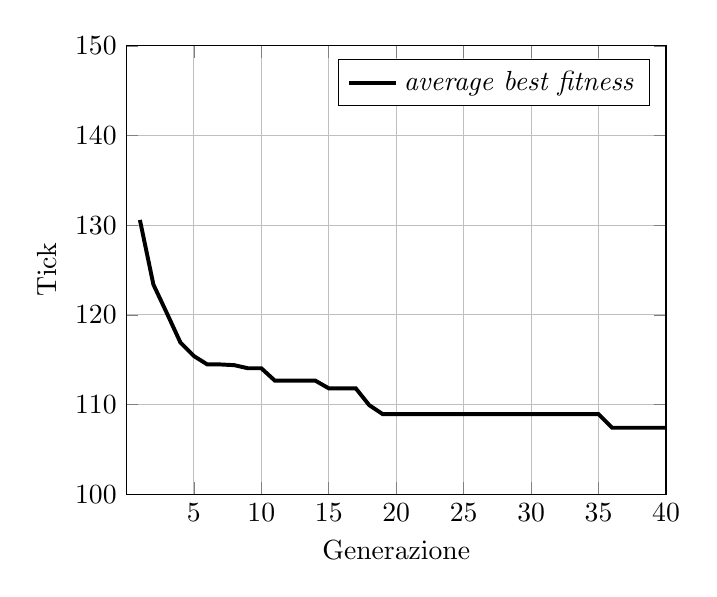
\begin{tikzpicture}
                \begin{axis}[
                    title={},
                    xlabel={Generazione},
                    ylabel={Tick},
                    xmin=0, xmax=40,
                    ymin=100, ymax=150,
                    xtick={5,10,15,20,25,30,35,40},
                    ytick={100,110,120,130,140,150},
                    legend pos=north east,
                    grid=major,
                    %ymajorgrids=true,
                    %xmajorgrids=true
                    %grid style=dashed,
                ]
                
                \addplot[
                    color=black,
                    line width=0.5mm,
                    ]
                    coordinates {
                        (1,130.58)(2,123.38)(3,120.18)(4,116.92)(5,115.4)(6,114.46)(7,114.46)(8,114.38)(9,114.04)(10,114.04)(11,112.66)(12,112.66)(13,112.66)(14,112.66)(15,111.8)(16,111.8)(17,111.8)(18,109.92)(19,108.92)(20,108.92)(21,108.92)(22,108.92)(23,108.92)(24,108.92)(25,108.92)(26,108.92)(27,108.92)(28,108.92)(29,108.92)(30,108.92)(31,108.92)(32,108.92)(33,108.92)(34,108.92)(35,108.92)(36,107.4)(37,107.4)(38,107.4)(39,107.4)(40,107.4)
                    };
                
                    \legend{\textit{average best fitness}}
                
                \end{axis}
            \end{tikzpicture}
        }
    \end{center}
    \caption{Ottimizzazione parametrica con Differential Evolution della strategia esplorativa di Sciadro 3.1, andamento della media tra le migliori fitness function delle 5 esecuzioni, al variare della generazione}
    \label{fitness_sciadro_dump}
\end{figure}   

\begin{table}[H]
    \centering
    
    \begin{tabular}{|l|c|}
    \hline
    \textbf{Algorithm}              & \textbf{Performance (tick)}              \\ \hline
    Esplorazione Sciadro 3.2        & $107.40 \; \pm \; 3.10$           \\ \hline
    \end{tabular}%
    
    \caption{Valutazione delle performance registrate dall'algoritmo di esplorazione di Sciadro 3.2.}
    \label{tabella_performance_dump}
\end{table}

\subsection{Adattamento dell'algoritmo di esplorazione di ACO}

La configurazione dei parametri tecnologici utilizzata per questa strategia è riassunta nella tabella \ref{tabella_parametri_dump_ACO}.
Per un'analisi dettagliata su tali parametri vedere il paragrafo \ref{esplorazione_paper}.

\begin{table}[H]
    \centering
    
    \begin{tabular}{|l|c|}
    \hline
    \textbf{Parameter}                      & \textbf{Value}        \\ \hline
    Wireless range                          & $100$                 \\ \hline
    $\beta_{0}$                             & $0.5$                 \\ \hline
    $\alpha$                                & $0.2$                 \\ \hline
    Inertial weight                         & $0.729$               \\ \hline
    Acceleration coefficient                & $2$                   \\ \hline
    \end{tabular}%
    
    \caption{Configurazione parametrica della tecnologia utilizzata nella fase sperimentale dello scenario \textit{Illegal Dump}.}
    \label{tabella_parametri_dump_ACO}
\end{table}

\subsubsection{Ottimizzazione parametrica con Differential Evolution}

Come previsto dall'algoritmo di \textit{Differential Evolution}, è necessario impostare degli intervalli che tale algoritmo utilizzerà durante l'ottimizzazione.
Sono stati definiti intervalli ampi per esplorare al meglio l'iperspazio definito dagli stessi.
In questo modo, infatti, si da più libertà all'algoritmo di DE di spaziare nella ricerca del minimo globale.

Lo schema riassuntivo degli intervalli utilizzato per la fase di ottimizzazione parametrica, nel caso della strategia di esplorazione \textit{ACO}, è presentato nella tabella \ref{tabella_intervalli_dump_ACO}

\begin{table}[H]
    \centering
    
    \begin{tabular}{|l|c|}
    \hline
    \textbf{Parameter}              & \textbf{Interval}         \\ \hline
    repulsiveStartIntensity         & $[0,100]$                 \\ \hline
    sensingRange                    & $[0,100]$                 \\ \hline
    EvaporationRateTimeUnit         & $[0,1]$                   \\ \hline
    $a_{1}$                         & $[0,2]$                   \\ \hline
    $a_{2}$                         & $[0,2]$                   \\ \hline
    $\phi$                          & $[0,2]$                   \\ \hline
    $\eta$                          & $[0,2]$                   \\ \hline
    $\lambda$                       & $[0,2]$                   \\ \hline
    \end{tabular}%
    
    \caption{Configurazione degli intervalli per l'ottimizzazione parametrica, attraverso l'algoritmo di \textit{Differential Evolution}, utilizzata nella fase sperimentale dello scenario \textit{Illegal Dump}.}
    \label{tabella_intervalli_dump_ACO}
\end{table}

Anche in questo caso, l'obiettivo è quello di effettuare un'analisi comparativa con le strategie utilizzate in precedenza.
A tal fine sono stati utilizzati gli stessi valori sia per il tasso di mutazione $F$ che per strategia e coefficiente di crossover $CR$.
In particolare:
\begin{itemize}
    \item \textit{Strategia di crossover:} DE/rand/1/bin;
    \item \textit{Tasso di mutazione:} $F=0.7$;
    \item \textit{Coefficiente di crossover:} $CR=0.5$
\end{itemize}

\subsubsection{Risultati sperimentali}

L'algoritmo di coordinamento esplorativo dello sciame è stato testato sullo scenario \textit{Illegal Dump}, con la seguente strategia:
\begin{itemize}
    \item \textit{5 esecuzioni dell'algoritmo di Differential evolution;}
    \item \textit{3 ripetizione della simulazione per ogni elemento della popolazione;}
    \item \textit{Fitness function:} $f(x) = \# tick[95 \% \; target_{found}]$
\end{itemize}

\begin{figure}[H] 
    \captionsetup{justification=centering, margin=2cm, font=footnotesize}
    \begin{center}
        \makebox[0.5\paperwidth]{
            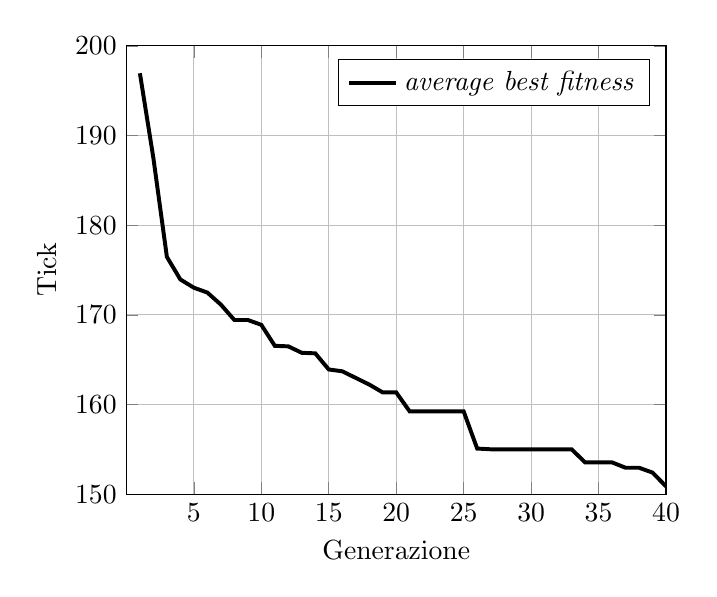
\begin{tikzpicture}
                \begin{axis}[
                    title={},
                    xlabel={Generazione},
                    ylabel={Tick},
                    xmin=0, xmax=40,
                    ymin=150, ymax=200,
                    xtick={5,10,15,20,25,30,35,40},
                    ytick={150,160,170,180,190,200},
                    legend pos=north east,
                    grid=major,
                    %ymajorgrids=true,
                    %xmajorgrids=true
                    %grid style=dashed,
                ]
                
                \addplot[
                    color=black,
                    line width=0.5mm,
                    ]
                    coordinates {
                        (1,196.94)(2,187.48)(3,176.46)(4,173.94)(5,173.02)(6,172.48)(7,171.14)(8,169.42)(9,169.42)(10,168.88)(11,166.54)(12,166.48)(13,165.76)(14,165.7)(15,163.9)(16,163.7)(17,162.96)(18,162.22)(19,161.34)(20,161.34)(21,159.22)(22,159.22)(23,159.22)(24,159.22)(25,159.22)(26,155.08)(27,155)(28,155)(29,155)(30,155)(31,155)(32,155)(33,155)(34,153.54)(35,153.54)(36,153.54)(37,152.94)(38,152.94)(39,152.4)(40,150.86)
                    };
                
                    \legend{\textit{average best fitness}}
                
                \end{axis}
            \end{tikzpicture}
        }
    \end{center}
    \caption{Ottimizzazione parametrica con Differential Evolution della strategia esplorativa ACO, andamento della media tra le migliori fitness function delle 5 esecuzioni, al variare della generazione}
    \label{fitness_ACO_dump}
\end{figure}   

\begin{table}[H]
    \centering
    
    \begin{tabular}{|l|c|}
    \hline
    \textbf{Algorithm}              & \textbf{Performance (tick)}              \\ \hline
    Esplorazione ACO                & $161.34 \; \pm \; 6.21$           \\ \hline
    \end{tabular}%
    
    \caption{Valutazione delle performance registrate dall'algoritmo di esplorazione ACO.}
    \label{tabella_performance_dump_ACO}
\end{table}


\subsection{Adattamento dell'algoritmo di reclutamento di Sciadro 3.2}

La strategia di reclutamento prevede una fase di lavorazione del target successiva alla scoperta dello stesso.
In questo caso, infatti, perché un target diventi \textit{Executed} è necessario che un numero minimo di droni si avvicini al target per l'esecuzione del task previsto dalla missione.

La configurazione dei parametri tecnologici utilizzata corrisponde con quella già introdotta nella sezione \ref{paragrafo_esplorazione_sciadro}.
L'unica differenza con il suddetto approccio di esplorazione è il parametro relativo al numero di droni necessario alla lavorazione del target, indicato con \textit{requiredDrones}.
Nelle fase sperimentale presentata di seguito $requiredDrones = 2$.

\subsubsection{Ottimizzazione parametrica con Differential Evolution}

Lo schema riassuntivo degli intervalli utilizzato nell'esecuzione dell'algoritmo di DE è presentato nella tabella \ref{tabella_intervalli_dump_sciadro32}

\begin{table}[H]
    \centering
    
    \begin{tabular}{|l|c|}
    \hline
    \textbf{Parameter}              & \textbf{Interval}                 \\ \hline
    radiusTop                       & $[1,13]$                          \\ \hline
    radiusDown                      & $[13,19]$                         \\ \hline
    evapRate                        & $[0.01,0.1]$                      \\ \hline
    olfaction                       & $[1,10]$                          \\ \hline
    flockAngle                      & $[15,45]$                         \\ \hline
    wiggleVar                       & $[5,15]$                          \\ \hline
    radiusSeparate                  & $[6,16]$                          \\ \hline
    maxSeparateTurn                 & $[30,45]$                         \\ \hline
    radiusAlign                     & $[16,22]$                         \\ \hline
    maxAlignTurn                    & $[30,45]$                         \\ \hline
    radiusCohere                    & $[18,26]$                         \\ \hline
maxCohereTurn                       & $[15,30]$                         \\ \hline
    \end{tabular}%
    
    \caption{Configurazione degli intervalli per l'ottimizzazione parametrica, attraverso l'algoritmo di \textit{Differential Evolution}, utilizzata nella fase sperimentale dello scenario \textit{Illegal Dump}.}
    \label{tabella_intervalli_dump_sciadro32}
\end{table}

Gli iperparametri $F$ e $CR$, per le fasi di mutazione e crossover dell'algoritmo di DE, e la strategia di crossover utilizzati sono illustrati di seguito:
\begin{itemize}
    \item \textit{Strategia di crossover:} DE/rand/1/bin;
    \item \textit{Tasso di mutazione:} $F=0.7$;
    \item \textit{Coefficiente di crossover:} $CR=0.5$
\end{itemize}

\subsubsection{Risultati sperimentali}

L'algoritmo di reclutamento è stato testato sullo scenario \textit{Illegal Dump}, con la seguente strategia:
\begin{itemize}
    \item \textit{5 esecuzioni dell'algoritmo di Differential evolution;}
    \item \textit{3 ripetizione della simulazione per ogni elemento della popolazione;}
    \item \textit{Fitness function:} $f(x) = \# tick[95 \% \; target_{executed}]$
\end{itemize}

\begin{figure}[H] 
    \captionsetup{justification=centering, margin=2cm, font=footnotesize}
    \begin{center}
        \makebox[0.5\paperwidth]{
            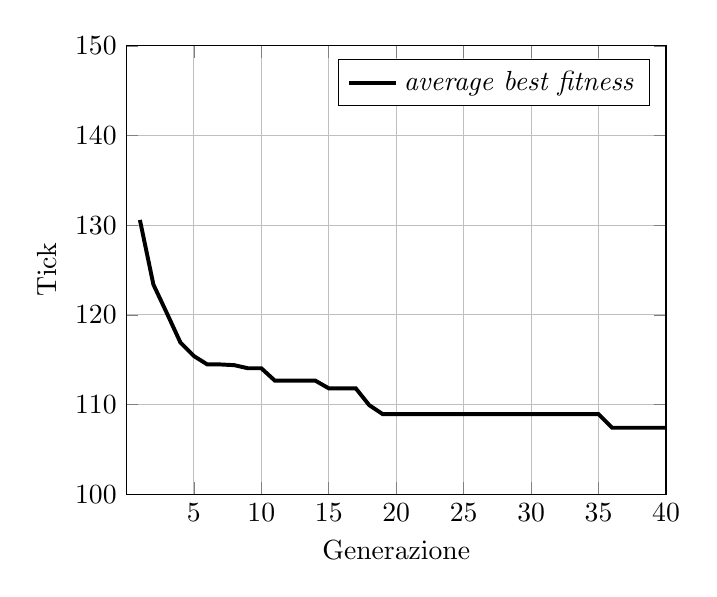
\begin{tikzpicture}
                \begin{axis}[
                    title={},
                    xlabel={Generazione},
                    ylabel={Tick},
                    xmin=0, xmax=40,
                    ymin=100, ymax=150,
                    xtick={5,10,15,20,25,30,35,40},
                    ytick={100,110,120,130,140,150},
                    legend pos=north east,
                    grid=major,
                    %ymajorgrids=true,
                    %xmajorgrids=true
                    %grid style=dashed,
                ]
                
                \addplot[
                    color=black,
                    line width=0.5mm,
                    ]
                    coordinates {
                        (1,130.58)(2,123.38)(3,120.18)(4,116.92)(5,115.4)(6,114.46)(7,114.46)(8,114.38)(9,114.04)(10,114.04)(11,112.66)(12,112.66)(13,112.66)(14,112.66)(15,111.8)(16,111.8)(17,111.8)(18,109.92)(19,108.92)(20,108.92)(21,108.92)(22,108.92)(23,108.92)(24,108.92)(25,108.92)(26,108.92)(27,108.92)(28,108.92)(29,108.92)(30,108.92)(31,108.92)(32,108.92)(33,108.92)(34,108.92)(35,108.92)(36,107.4)(37,107.4)(38,107.4)(39,107.4)(40,107.4)
                    };
                
                    \legend{\textit{average best fitness}}
                
                \end{axis}
            \end{tikzpicture}
        }
    \end{center}
    \caption{Ottimizzazione parametrica con Differential Evolution della strategia esplorativa di Sciadro 3.1, andamento della media tra le migliori fitness function delle 5 esecuzioni, al variare della generazione}
    \label{fitness_sciadro_dump}
\end{figure}   

\begin{table}[H]
    \centering
    
    \begin{tabular}{|l|c|}
    \hline
    \textbf{Algorithm}              & \textbf{Performance (tick)}              \\ \hline
    Reclutamento Sciadro 3.2                     & $107.40 \; \pm \; 3.10$           \\ \hline
    \end{tabular}%
    
    \caption{Valutazione delle performance registrate dall'algoritmo di reclutamento di Sciadro 3.2.}
    \label{tabella_performance_dump}
\end{table}

\section{Scenario \textit{Rural Mine}}

Lo scenario è statico: \textit{Rural Mine} si basa su dati di pubblico dominio relativi a mine antiuomo presenti in aree extraurbane vicino Sarajevo, Bosnia-Herzegovina \cite{seedemining2018}.
Di seguito sono riportate le caratteristiche dello scenario:

\begin{itemize}
    \item \textit{Area in metri:} 400 x 400
    \item \textit{Area in patch:} 201 x 201
    \item \textit{Dimensione patch:} 1.99m x 1.99m
    \item \textit{Conversione spaziale:} 1 m = 0.502 patch
    \item \textit{Conversione temporale:} 1 s = 1 tick
    \item \textit{Numero target statici presenti nell'area:} 28
    \item \textit{Numero target dinamici presenti nell'area:} 0
    \item \textit{Numero ostacoli presenti nell'area:} 285
    \item \textit{Flotta utilizzata:} 80 droni
\end{itemize}

Lo scenario presenta solo target statici, di conseguenza la funzione obiettivo è rappresentata dal tempo di rilevamento del $95 \%$ dei target.

Per osservarne la complessità ambientale, le figure \ref{ruralMine_map} e \ref{ruralMine_scenario} mostrano la mappa satellitare utilizzata per \textit{Rural Mine}, e la corrispondente immagine vettoriale iniziale rappresentata nell'ambiente di simulazione, rispettivamente. 
Gli ostacoli  sono rappresentati in grigio, mentre i bersagli sono rappresentati come 'x' nere. 
I droni sono posizionati agli angoli e sono orientati verso il centro dell'area.

\begin{figure}[H] 
    \captionsetup{justification=centering, margin=2cm, font=footnotesize}
    \begin{center}
    \makebox[\textwidth]{\includegraphics[width=0.3\paperwidth]{img/ruralMine_map.png}}
    \end{center}
    \caption{Immagine satellitare dello scenario Rural Mine.}
    \label{ruralMine_map}
\end{figure}

\begin{figure}[H] 
    \captionsetup{justification=centering, margin=2cm, font=footnotesize}
    \begin{center}
    \makebox[\textwidth]{\includegraphics[width=0.3\paperwidth]{img/ruralMine_scenario.png}}
    \end{center}
    \caption{Immagine vettoriale dello scenario Rural Mine.}
    \label{ruralMine_scenario}
\end{figure}

La configurazione dei parametri tecnologici utilizzata nella fase sperimentale dello scenario \textit{Rural Mine} è  riassunta nella tabella \ref{tabella_parametri_ruralMine}.

\begin{table}[H]
    \centering
    
    \begin{tabular}{|l|c|}
    \hline
    \textbf{Parameter}              & \textbf{Value}                \\ \hline
    Radius                          & $0.2 \; patch$                \\ \hline
    Max speed                       & $8.5 \; patch/tick$           \\ \hline
    Cruising speed                  & $2 \; patch/tick$             \\ \hline
    Max acceleration                & $2 \; patch/tick^{2}$         \\ \hline
    Max deceleration                & $-2 \; patch/tick^{2}$        \\ \hline
    Max angular speed               & $2.6 \; rad/s$                \\ \hline
    Max angular acceleration        & $7 \; rad/s^{2}$              \\ \hline
    Max angular deceleration        & $-7 \; rad/s^{2}$             \\ \hline
    Battery duration                & $1440 \; tick$                \\ \hline
    Sensing radius                  & $2.5 \; patch$                \\ \hline
    Sensing angle                   & \ang{360}                        \\ \hline
    Reachable radius                & $4 \; patch$                  \\ \hline
    Reachable angle                 & \ang{360}                        \\ \hline
    Obstacle vision distance        & $6 \; patch$                  \\ \hline
    Obstacle vision angle           & \ang{60}                        \\ \hline
    Gap angle                       & \ang{20}                        \\ \hline
    \end{tabular}%
    
    \caption{Configurazione parametrica della tecnologia utilizzata nella fase sperimentale dello scenario \textit{Rural Mine}.}
    \label{tabella_parametri_ruralMine}
\end{table}

\subsection{Ottimizzazione parametrica con Differential Evolution}

Uno schema riassuntivo degli intervalli utilizzati per la fase di ottimizzazione parametrica attraverso l'algoritmo di \textit{Differential Evolution} è presentato nella tabella \ref{tabella_intervalli_ruralMine}

\begin{table}[H]
    \centering
    
    \begin{tabular}{|l|c|}
    \hline
    \textbf{Parameter}              & \textbf{Interval}                 \\ \hline
    radiusTop                       & $[1,13]$                          \\ \hline
    radiusDown                      & $[13,19]$                         \\ \hline
    evapRate                        & $[0.01,0.1]$                      \\ \hline
    olfaction                       & $[1,10]$                          \\ \hline
    flockAngle                      & $[15,45]$                         \\ \hline
    wiggleVar                       & $[5,15]$                          \\ \hline
    radiusSeparate                  & $[6,16]$                          \\ \hline
    maxSeparateTurn                 & $[30,45]$                         \\ \hline
    radiusAlign                     & $[16,22]$                         \\ \hline
    maxAlignTurn                    & $[30,45]$                         \\ \hline
    radiusCohere                    & $[18,26]$                         \\ \hline
    maxCohereTurn                       & $[15,30]$                         \\ \hline
    \end{tabular}%
    
    \caption{Configurazione degli intervalli per l'ottimizzazione parametrica, attraverso l'algoritmo di \textit{Differential Evolution}, utilizzata nella fase sperimentale dello scenario \textit{Rural Mine}.}
    \label{tabella_intervalli_ruralMine}
\end{table}

I valori relativi agli iperparametri sono i seguenti:
\begin{itemize}
    \item \textit{Strategia di crossover:} DE/rand/1/bin;
    \item \textit{Tasso di mutazione:} $F=0.7$;
    \item \textit{Coefficiente di crossover:} $CR=0.5$
\end{itemize}

\subsection{Risultati sperimentali}

L'algoritmo di coordinamento dello sciame è stato testato sullo scenario \textit{Rural Mine}, con la seguente strategia:
\begin{itemize}
    \item \textit{5 esecuzioni dell'algoritmo di Differential evolution;}
    \item \textit{3 ripetizione della simulazione per ogni elemento della popolazione;}
    \item \textit{Fitness function:} $f(x) = \# tick[95 \% \; target_{found}]$
\end{itemize}

\begin{figure}[H] 
    \captionsetup{justification=centering, margin=2cm, font=footnotesize}
    \begin{center}
        \makebox[0.5\paperwidth]{
            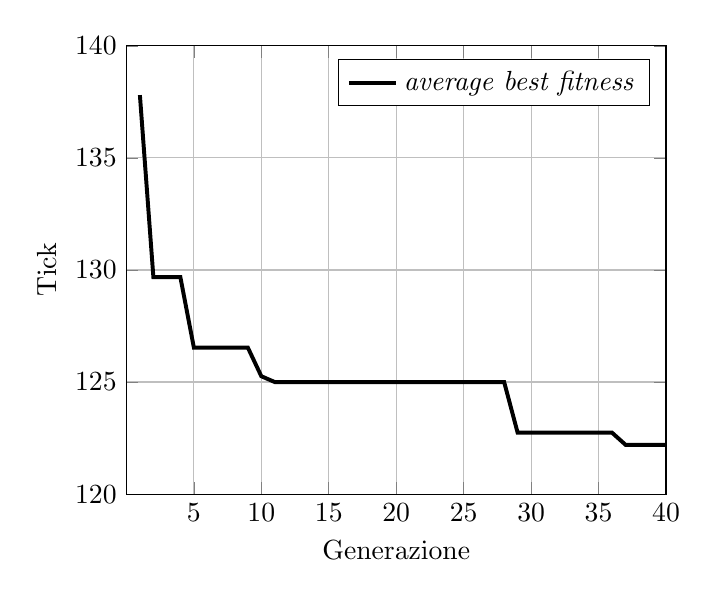
\begin{tikzpicture}
                \begin{axis}[
                    title={},
                    xlabel={Generazione},
                    ylabel={Tick},
                    xmin=0, xmax=40,
                    ymin=120, ymax=140,
                    xtick={5,10,15,20,25,30,35,40},
                    ytick={120,125,130,135,140},
                    legend pos=north east,
                    grid=major,
                    %ymajorgrids=true,
                    %xmajorgrids=true
                    %grid style=dashed,
                ]
                
                \addplot[
                    color=black,
                    line width=0.5mm,
                    ]
                    coordinates {
                        (1,137.8)(2,129.68)(3,129.68)(4,129.68)(5,126.54)(6,126.54)(7,126.54)(8,126.54)(9,126.54)(10,125.26)(11,125)(12,125)(13,125)(14,125)(15,125)(16,125)(17,125)(18,125)(19,125)(20,125)(21,125)(22,125)(23,125)(24,125)(25,125)(26,125)(27,125)(28,125)(29,122.74)(30,122.74)(31,122.74)(32,122.74)(33,122.74)(34,122.74)(35,122.74)(36,122.74)(37,122.2)(38,122.2)(39,122.2)(40,122.2)
                    };
                
                    \legend{\textit{average best fitness}}
                
                \end{axis}
            \end{tikzpicture}
        }
    \end{center}
    \caption{Ottimizzazione parametrica con Differential Evolution, andamento della media tra le migliori fitness function delle 5 esecuzioni, al variare della generazione}
    \label{fitness_sciadro_ruralMine}
\end{figure}   

\begin{table}[H]
    \centering
    
    \begin{tabular}{|l|c|}
    \hline
    \textbf{Algorithm}              & \textbf{Performance (tick)}       \\ \hline
    Sciadro 3.1                     & $125.96 \; \pm \; 8.90$           \\ \hline
    Sciadro 3.2                     & $122.20 \; \pm \; 3.89$           \\ \hline
    \end{tabular}%
    
    \caption{Analisi comparativa delle performance.}
    \label{tabella_performance_ruralMine}
\end{table}

\section{Scenario \textit{Urban Mine}}

Lo scenario è statico: \textit{Urban Mine} si basa su dati di pubblico dominio relativi a mine antiuomo presenti in aree urbane vicino Sarajevo, Bosnia-Herzegovina \cite{seedemining2018}.
Di seguito sono riportate le caratteristiche dello scenario:

\begin{itemize}
    \item \textit{Area in metri:} 400 x 400
    \item \textit{Area in patch:} 201 x 201
    \item \textit{Dimensione patch:} 1.99m x 1.99m
    \item \textit{Conversione spaziale:} 1 m = 0.502 patch
    \item \textit{Conversione temporale:} 1 s = 1 tick
    \item \textit{Numero target statici presenti nell'area:} 40
    \item \textit{Numero target dinamici presenti nell'area:} 0
    \item \textit{Numero ostacoli presenti nell'area:} 3664
    \item \textit{Flotta utilizzata:} 80 droni
\end{itemize}

Lo scenario presenta solo target statici, di conseguenza la funzione obiettivo è rappresentata dal tempo di rilevamento del $95 \%$ dei target.

Per osservarne la complessità ambientale, le figure \ref{urbanMine_map} e \ref{urbanMine_scenario} mostrano la mappa satellitare utilizzata per \textit{Urban Mine}, e la corrispondente immagine vettoriale iniziale rappresentata nell'ambiente di simulazione, rispettivamente. 
Gli ostacoli  sono rappresentati in grigio, mentre i bersagli sono rappresentati come 'x' nere. 
I droni sono posizionati agli angoli e sono orientati verso il centro dell'area.

\begin{figure}[H] 
    \captionsetup{justification=centering, margin=2cm, font=footnotesize}
    \begin{center}
    \makebox[\textwidth]{\includegraphics[width=0.3\paperwidth]{img/urbanMine_map.png}}
    \end{center}
    \caption{Immagine satellitare dello scenario Urban Mine.}
    \label{urbanMine_map}
\end{figure}

\begin{figure}[H] 
    \captionsetup{justification=centering, margin=2cm, font=footnotesize}
    \begin{center}
    \makebox[\textwidth]{\includegraphics[width=0.3\paperwidth]{img/urbanMine_scenario.png}}
    \end{center}
    \caption{Immagine vettoriale dello scenario Urban Mine.}
    \label{urbanMine_scenario}
\end{figure}

La configurazione dei parametri tecnologici utilizzata nella fase sperimentale dello scenario \textit{Urban Mine} è  riassunta nella tabella \ref{tabella_parametri_urbanMine}.

\begin{table}[H]
    \centering
    
    \begin{tabular}{|l|c|}
    \hline
    \textbf{Parameter}              & \textbf{Value}                \\ \hline
    Radius                          & $0.2 \; patch$                \\ \hline
    Max speed                       & $8.5 \; patch/tick$           \\ \hline
    Cruising speed                  & $2 \; patch/tick$             \\ \hline
    Max acceleration                & $2 \; patch/tick^{2}$         \\ \hline
    Max deceleration                & $-2 \; patch/tick^{2}$        \\ \hline
    Max angular speed               & $2.6 \; rad/s$                \\ \hline
    Max angular acceleration        & $7 \; rad/s^{2}$              \\ \hline
    Max angular deceleration        & $-7 \; rad/s^{2}$             \\ \hline
    Battery duration                & $1440 \; tick$                \\ \hline
    Sensing radius                  & $2.5 \; patch$                \\ \hline
    Sensing angle                   & \ang{360}                        \\ \hline
    Reachable radius                & $4 \; patch$                  \\ \hline
    Reachable angle                 & \ang{360}                        \\ \hline
    Obstacle vision distance        & $6 \; patch$                  \\ \hline
    Obstacle vision angle           & \ang{60}                        \\ \hline
    Gap angle                       & \ang{20}                        \\ \hline
    \end{tabular}%
    
    \caption{Configurazione parametrica della tecnologia utilizzata nella fase sperimentale dello scenario \textit{Urban Mine}.}
    \label{tabella_parametri_urbanMine}
\end{table}

\subsection{Ottimizzazione parametrica con Differential Evolution}

Uno schema riassuntivo degli intervalli utilizzati per la fase di ottimizzazione parametrica attraverso l'algoritmo di \textit{Differential Evolution} è presentato nella tabella \ref{tabella_intervalli_urbanMine}

\begin{table}[H]
    \centering
    
    \begin{tabular}{|l|c|}
    \hline
    \textbf{Parameter}              & \textbf{Interval}                 \\ \hline
    radiusTop                       & $[1,13]$                          \\ \hline
    radiusDown                      & $[13,19]$                         \\ \hline
    evapRate                        & $[0.01,0.1]$                      \\ \hline
    olfaction                       & $[1,10]$                          \\ \hline
    flockAngle                      & $[15,45]$                         \\ \hline
    wiggleVar                       & $[5,15]$                          \\ \hline
    radiusSeparate                  & $[6,16]$                          \\ \hline
    maxSeparateTurn                 & $[30,45]$                         \\ \hline
    radiusAlign                     & $[16,22]$                         \\ \hline
    maxAlignTurn                    & $[30,45]$                         \\ \hline
    radiusCohere                    & $[18,26]$                         \\ \hline
    maxCohereTurn                       & $[15,30]$                         \\ \hline
    \end{tabular}%
    
    \caption{Configurazione degli intervalli per l'ottimizzazione parametrica, attraverso l'algoritmo di \textit{Differential Evolution}, utilizzata nella fase sperimentale dello scenario \textit{Urban Mine}.}
    \label{tabella_intervalli_urbanMine}
\end{table}

I valori relativi agli iperparametri sono i seguenti:
\begin{itemize}
    \item \textit{Strategia di crossover:} DE/rand/1/bin;
    \item \textit{Tasso di mutazione:} $F=0.7$;
    \item \textit{Coefficiente di crossover:} $CR=0.5$
\end{itemize}

\subsection{Risultati sperimentali}

L'algoritmo di coordinamento dello sciame è stato testato sullo scenario \textit{Urban Mine}, con la seguente strategia:
\begin{itemize}
    \item \textit{5 esecuzioni dell'algoritmo di Differential evolution;}
    \item \textit{3 ripetizione della simulazione per ogni elemento della popolazione;}
    \item \textit{Fitness function:} $f(x) = \# tick[95 \% \; target_{found}]$
\end{itemize}

\begin{figure}[H] 
    \captionsetup{justification=centering, margin=2cm, font=footnotesize}
    \begin{center}
        \makebox[0.5\paperwidth]{
            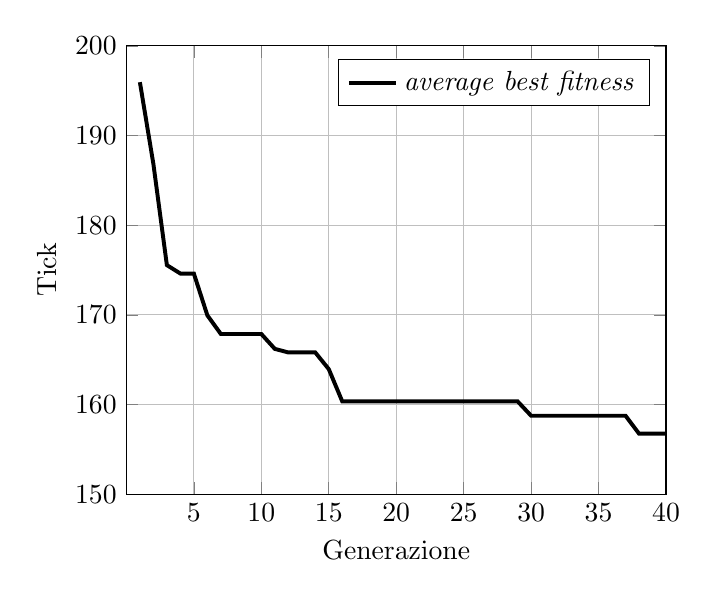
\begin{tikzpicture}
                \begin{axis}[
                    title={},
                    xlabel={Generazione},
                    ylabel={Tick},
                    xmin=0, xmax=40,
                    ymin=150, ymax=200,
                    xtick={5,10,15,20,25,30,35,40},
                    ytick={150,160,170,180,190,200},
                    legend pos=north east,
                    grid=major,
                    %ymajorgrids=true,
                    %xmajorgrids=true
                    %grid style=dashed,
                ]
                
                \addplot[
                    color=black,
                    line width=0.5mm,
                    ]
                    coordinates {
                        (1,195.94)(2,186.82)(3,175.54)(4,174.6)(5,174.6)(6,169.94)(7,167.86)(8,167.86)(9,167.86)(10,167.86)(11,166.2)(12,165.8)(13,165.8)(14,165.8)(15,163.94)(16,160.34)(17,160.34)(18,160.34)(19,160.34)(20,160.34)(21,160.34)(22,160.34)(23,160.34)(24,160.34)(25,160.34)(26,160.34)(27,160.34)(28,160.34)(29,160.34)(30,158.74)(31,158.74)(32,158.74)(33,158.74)(34,158.74)(35,158.74)(36,158.74)(37,158.74)(38,156.74)(39,156.74)(40,156.74)
                    };
                
                    \legend{\textit{average best fitness}}
                
                \end{axis}
            \end{tikzpicture}
        }
    \end{center}
    \caption{Ottimizzazione parametrica con Differential Evolution, andamento della media tra le migliori fitness function delle 5 esecuzioni, al variare della generazione}
    \label{fitness_sciadro_urbanMine}
\end{figure}   

\begin{table}[H]
    \centering
    
    \begin{tabular}{|l|c|}
    \hline
    \textbf{Algorithm}              & \textbf{Performance (tick)}       \\ \hline
    Sciadro 3.1                     & $152.38 \; \pm \; 5.25$           \\ \hline
    Sciadro 3.2                     & $160.34 \; \pm \; 5.42$           \\ \hline
    \end{tabular}%
    
    \caption{Analisi comparativa delle performance.}
    \label{tabella_performance_urbanMine}
\end{table}

\newpage
\section{Analisi comparativa delle performance}

In questa sezione verrà presentato uno schema riassuntivo dei risultati ottenuti nella fase sperimentale, al fine di poter effettuare una comparazione tra le performance registrate dalle varie strategie adottate.

Per lo scenario \textit{Illegal Dump} sono state adattate entrambe le strategie di esplorazione introdotte nei capitoli precedenti e sono state confrontate con i risultati di altri studi presenti in letteratura.
La tabella \ref{analisi_comparativa_esplorazione_dump} mostra i risultati degli esperimenti realizzati.

\begin{table}[H]
    \centering
    
    \begin{tabular}{|l|c|}
    \hline
    \textbf{Algorithm}              & \textbf{Performance (tick)}       \\ \hline
    Sciadro 3.1                     & $121.70 \; \pm \; 4.75$           \\ \hline
    Sciadro 3.2                     & $107.40 \; \pm \; 3.10$           \\ \hline
    ACO                             & $161.34 \; \pm \; 6.21$           \\ \hline
    \end{tabular}%
    
    \caption{Strategia di esplorazione dello scenario \textit{Illegal Dump}, analisi comparativa delle performance.}
    \label{analisi_comparativa_esplorazione_dump}
\end{table}

Per gli scenari \textit{Rural Mine} e \textit{Urban Mine} si è scelto di adattare solo la strategia di esplorazione Sciadro 3.2, al fine di testarne le performance su scenari di diverse conformazioni.
Anche in questo caso si è scelto di valutare le performance del simulatore attraverso un confronto con le performance registrate, sugli stessi scenari, da Sciadro 3.1.
Le tabelle \ref{analisi_comparativa_esplorazione_ruralMine} e \ref{analisi_comparativa_esplorazione_urbanMine} mostrano i risultati degli esperimenti realizzati.

\begin{table}[H]
    \centering
    
    \begin{tabular}{|l|c|}
    \hline
    \textbf{Algorithm}              & \textbf{Performance (tick)}       \\ \hline
    Sciadro 3.1                     & $121.70 \; \pm \; 4.75$           \\ \hline
    Sciadro 3.2                     & $107.40 \; \pm \; 3.10$           \\ \hline
    \end{tabular}%
    
    \caption{Strategia di esplorazione dello scenario \textit{Rural Mine}, analisi comparativa delle performance.}
    \label{analisi_comparativa_esplorazione_ruralMine}
\end{table}

\begin{table}[H]
    \centering
    
    \begin{tabular}{|l|c|}
    \hline
    \textbf{Algorithm}              & \textbf{Performance (tick)}       \\ \hline
    Sciadro 3.1                     & $121.70 \; \pm \; 4.75$           \\ \hline
    Sciadro 3.2                     & $107.40 \; \pm \; 3.10$           \\ \hline
    \end{tabular}%
    
    \caption{Strategia di esplorazione dello scenario \textit{Urban Mine}, analisi comparativa delle performance.}
    \label{analisi_comparativa_esplorazione_urbanMine}
\end{table}